%%%%%%%%%%%%%%%%%%%%%%%%%%%%%%%%%%%%%%%%%%%%%%%%%%%%%%%%%%%%%%%%%%%%%%%%%%%%%%%%%
%
%  Diplomarbeit Vorname Name Datum         
%  "Titel"
%  Lehrstuhl fuer Mustererkennung, FAU Erlangen-Nuernberg
%
%%%%%%%%%%%%%%%%%%%%%%%%%%%%%%%%%%%%%%%%%%%%%%%%%%%%%%%%%%%%%%%%%%%%%%%%%%%%%%%%%

% ++ LME LateX Dokument 
%    Die Verwendung der option "german" bindet german.sty ein.
%    For english papers, use the "english" option and talk to your advisor.
%\documentclass[english,mt]{lmedoc}
\documentclass[english,mt]{lmedoc}

% ++ Umlaut Unterstuetzung
%    Paket "inputenc" kann verwendet werden, um z.B. Umlaute oder das scharfe S
%    direkt (als Nicht-ASCII-Zeichen) einzubinden. Dabei auf die korrekte
%    Kodiermethode achten (z.B. Linux: latin1)! 
\usepackage[latin1]{inputenc}

% ++ es werden keine underfull hboxes als Fehler ausgegeben,
%    da das ja nur hei�t, dass die Seite noch nicht ganz voll ist
\hbadness=10000



\includeonly{mt01, mt02, mt03, mt04, mt05, mt06, mt07, mt08, mt09, mt10, mt11, mt-lit, mt-lof, mt-lot}

\pagenumbering{roman}

%\bibliographystyle{galpha1a} %german bibliography
\bibliographystyle{alphamod} %english bibliography

\begin{document}
\clearpage
  \begin{deckblatt}
    \Titel{Determining the Influence of Papyrus Characteristics and Data Augmentation on Fragments Retrieval with Deep Metric Learning}
    \Name{Bohnstedt}
    \Vorname{Gunzenhause}
    \Geburtsort{Erlangen}
    \Geburtsdatum{17.02.1992}
    \Betreuer{Dr.-Ing.~V.~Christlein,  Prof.~Dr.-Ing.~habil.~A.~Maier, Mathias Seuret M. Sc.}
    \Start{Start}
    \Ende{Ende}
  \end{deckblatt}


\cleardoublepage


Ich versichere, dass ich die Arbeit ohne fremde Hilfe und ohne Benutzung
anderer als der angegebenen Quellen angefertigt habe und dass die Arbeit
in gleicher oder "ahnlicher Form noch keiner anderen Pr"ufungsbeh"orde
vorgelegen hat und von dieser als Teil einer Pr"ufungsleistung
angenommen wurde. Alle Ausf"uhrungen, die w"ortlich oder sinngem"a"s
"ubernommen wurden, sind als solche gekennzeichnet.
\\

Die Richtlinien des Lehrstuhls f"ur Studien- und Diplomarbeiten
habe ich gelesen und anerkannt, insbesondere die Regelung des
Nutzungsrechts. \\[15mm]
Erlangen, den \selectlanguage{german} \today \hspace{6.0cm} \\[10mm]

\selectlanguage{english} %remove this line for german style

\cleardoublepage

\begin{center}
\bfseries
"Ubersicht

Lorem Ipsum is simply dummy text of the printing and typesetting industry. Lorem Ipsum has been the industry's standard dummy text ever since the 1500s, when an unknown printer took a galley of type and scrambled it to make a type specimen book. It has survived not only five centuries, but also the leap into electronic typesetting, remaining essentially unchanged. It was popularised in the 1960s with the release of Letraset sheets containing Lorem Ipsum passages, and more recently with desktop publishing software like Aldus PageMaker including versions of Lorem Ipsu
\normalfont
\end{center}


\vspace{5.0cm}

\begin{center}
\bfseries
Abstract

Lorem Ipsum is simply dummy text of the printing and typesetting industry. Lorem Ipsum has been the industry's standard dummy text ever since the 1500s, when an unknown printer took a galley of type and scrambled it to make a type specimen book. It has survived not only five centuries, but also the leap into electronic typesetting, remaining essentially unchanged. It was popularised in the 1960s with the release of Letraset sheets containing Lorem Ipsum passages, and more recently with desktop publishing software like Aldus PageMaker including versions of Lorem Ipsu
\normalfont
\end{center}

\cleardoublepage

\tableofcontents

\cleardoublepage \pagenumbering{arabic}

\chapter{Introduction}
\label{chap:intro}
Ancient papyri are \cite{Pirrone21} frequently torn into several fragments, and the task of papyrologists is to assemble
and decipher these fragments. Once successfully reconstructed, ancient papyrus offers the opportunity
to gather crucial information about past times. However, reassembling by hand is time-consuming
because fragments differ in color, structure, and shape. Since the phrase puzzling is used, it implies that those fragments are perfectly designed puzzle pieces. Usually, it is the opposite. That means that non-professionals can not tell if two images belong together at all. An example is shown in Figure \ref{fig:papyri_sample}. It can be observed from the Figure that the fibers, the color, and the structure of the two fragments do not fit perfectly into each other. Nevertheless, they belong to the same papyrus. It is hard to tell whether fragments belong together or not because they age differently. Environmental local factors such as exposure to sunlight determine the altering process differently. For example, the medium color of two fragments is inconsistent if one fragment was buried and the second fragment was not. That implies that color is not a good feature for matching fragments.\\
Finding meaningful features (semi) automatically on historical documents and reassembling them has become a popular challenge in the computer vision community. The researchers apply machine learning algorithms to the data and train a model. Those models can then find potential matching candidates for a specific fragment.
\begin{figure}[t]
	\label{fig:papyri_sample}
	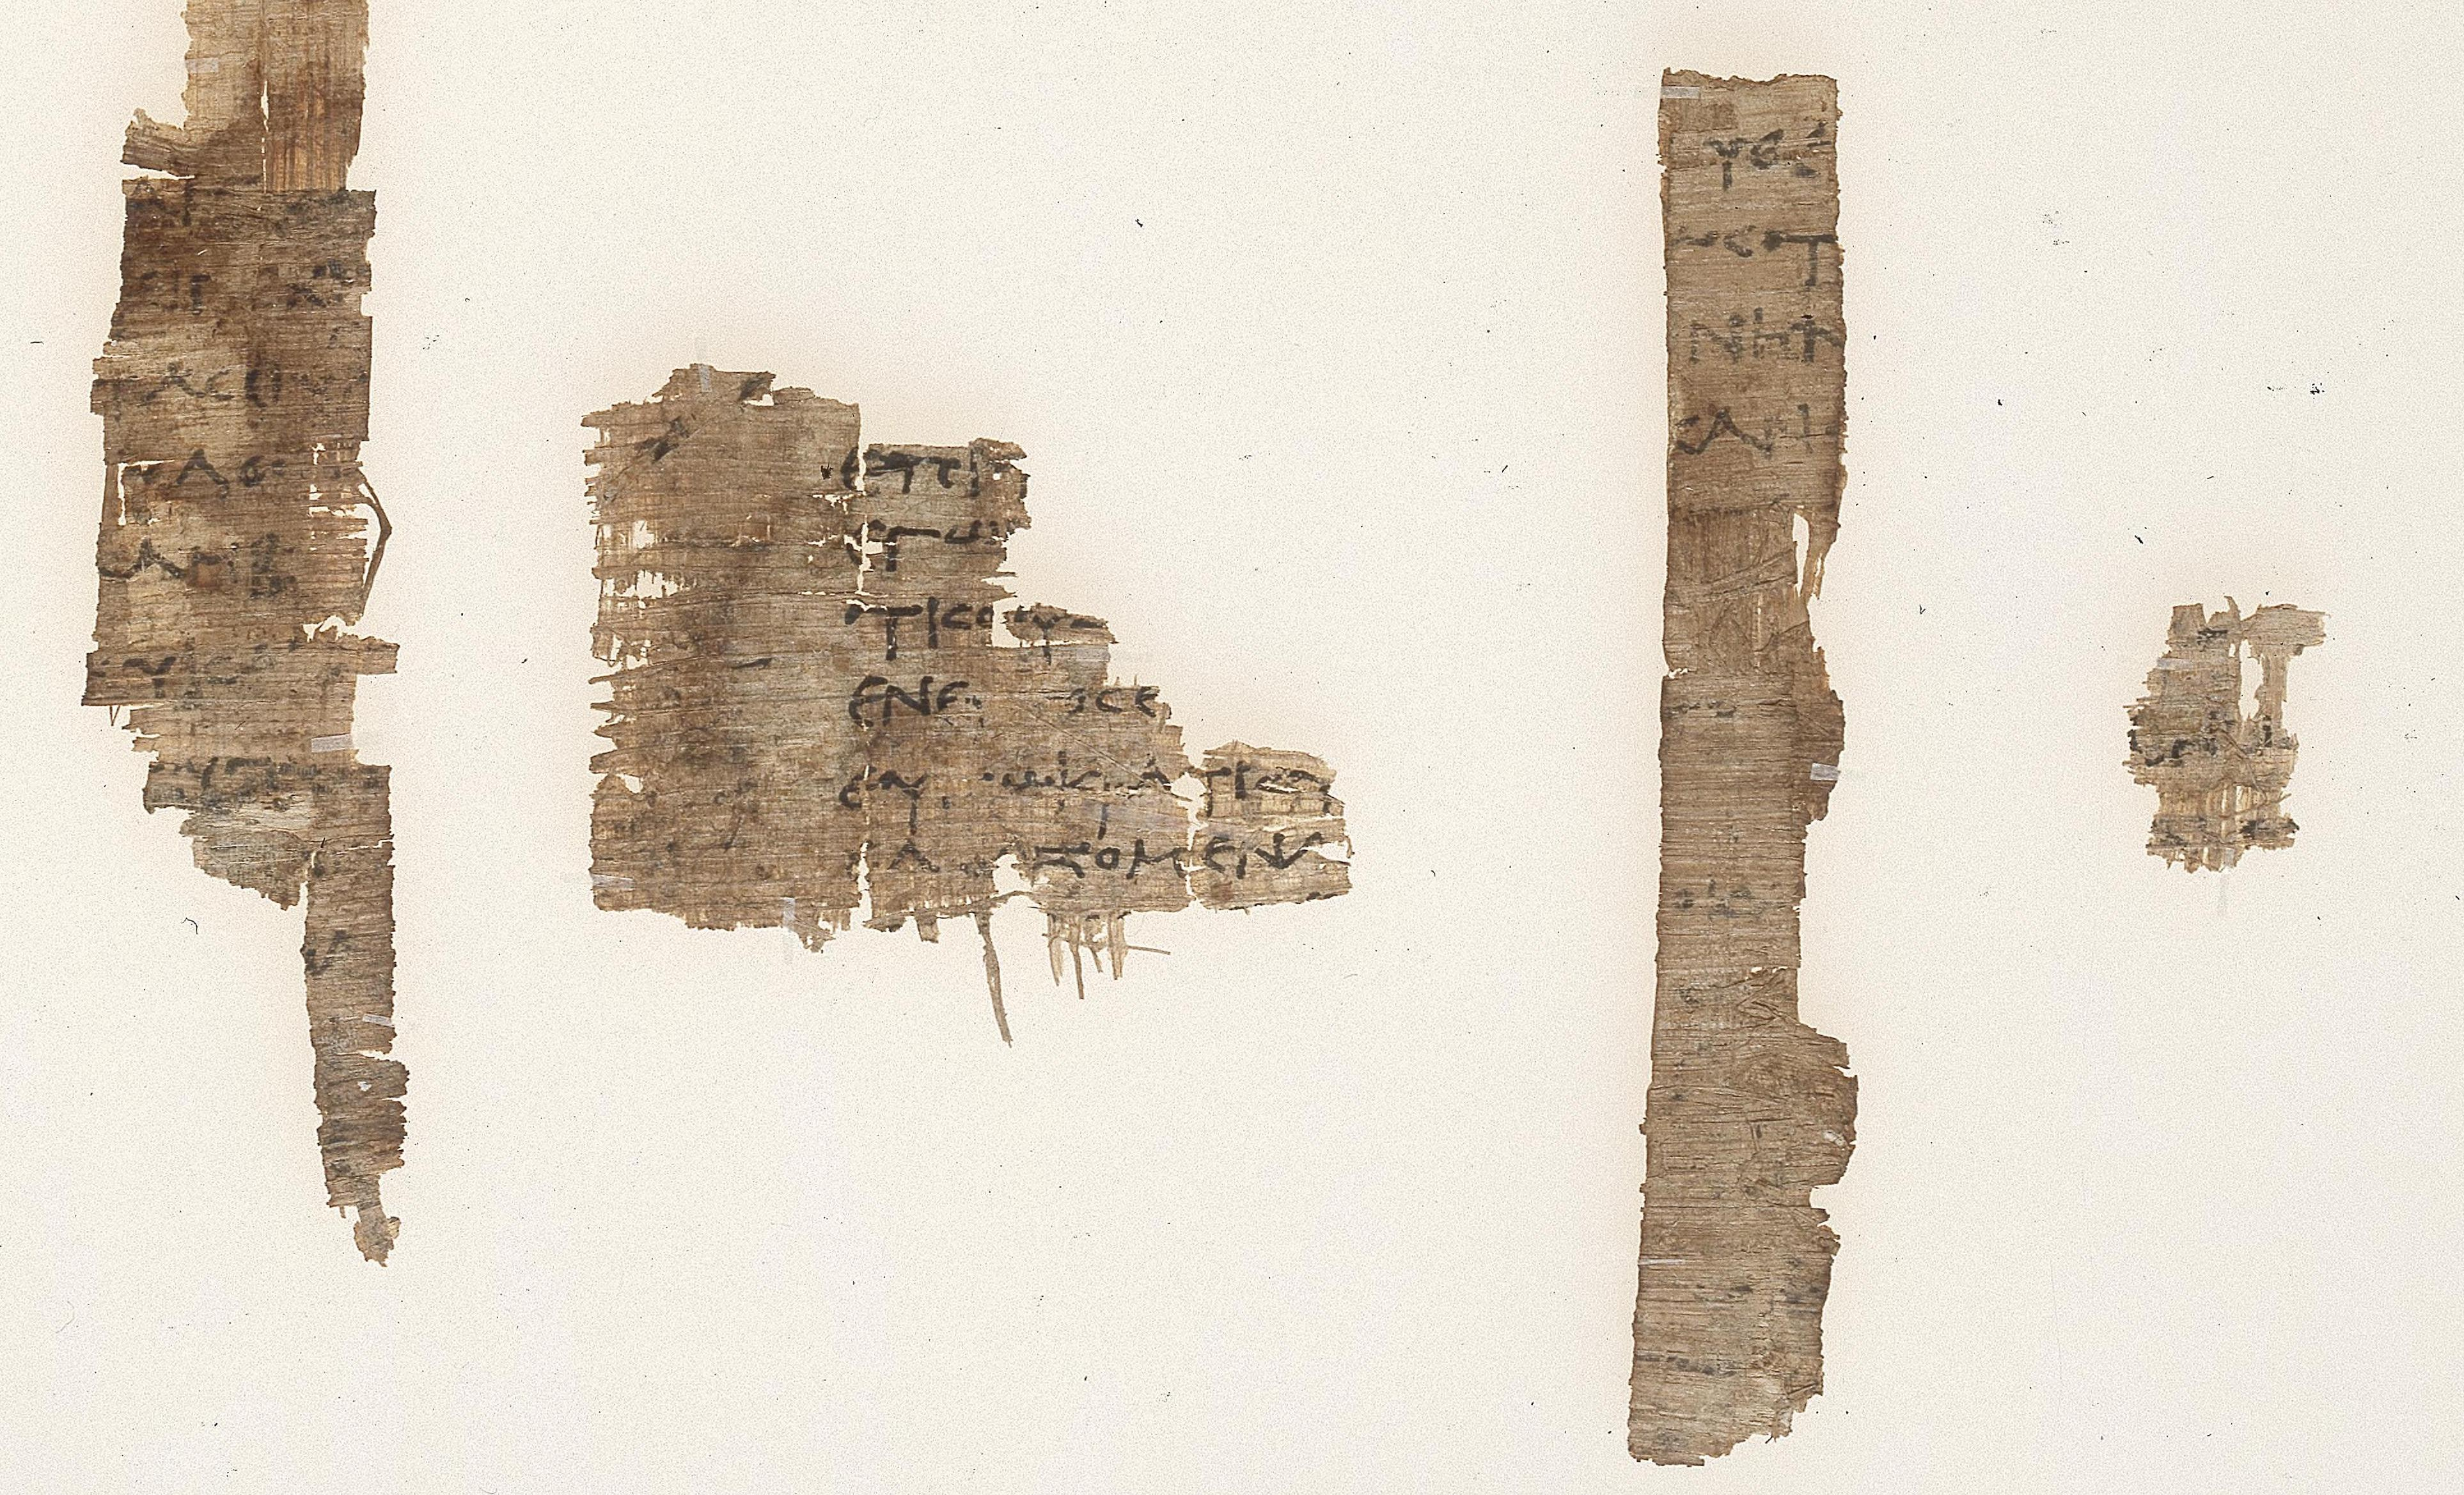
\includegraphics[width=\textwidth]{figures/papyri_sample.jpg}
	\caption{A papyri torn into several fragments}
\end{figure}
Deep Learning algorithms are among the commonly discussed types of algorithms when it comes to supporting papyrologists. Research has shown that the use of Deep Learning can increase the efficiency of papyrologists. However, even though the results are promising, there are still many unanswered questions that we do not understand. Once a better understanding of the features is obtained, the algorithms can increase the papyrologist's efficiency by a greater chance. 


\section{Contribution}
The general objective of this thesis is to make the work of papyrologists easier and increase their efficiency
by partially automating the reassembling process. To this end, an algorithm is designed to infer a
smaller sub-selection of fragments with a high likelihood of being a potential fit. In the following, this
algorithm is called puzzle-helper. Additionally, the thesis explores the use of papyrus fibers to determine an accurate spatial position of two potential matching fragments. Also, using deep learning implies that a vast amount of (labeled) data is required. The database from the University of Michigan offers plenty of it. Once the data is downloaded, it must be correctly preprocessed, like removing low contrast images or labeling the data. In particular, this thesis is centered around the following research questions:
\begin{questions}
	\item  Does the puzzle-helpers-accuracy differ significantly when only the text or only the fibers are used as input as opposed to the unprocessed data?	
	\item  With the help of papyrus fibers, is it possible to determine the position of a fragment out of several matching candidates?	
\end{questions}


\section{Outline}
In the Chapter \ref{chap:intro}, the context of this master thesis was explained, and the research questions got defined. In the following, it is explained how the thesis is structured. Chapter \ref{chap:stateArt} presents groundbreaking work in all areas that are relevant for this thesis. That includes binarization, inpainting, and deep metric learning. The chapter's goal is to show the reader a quick overview of actual results in the field of historical fragment retrieval. Chapter \ref{chap:puzzleHelper} aims to explain how a ground truth is computed with the help of Deep Metric Learning (DML) for comparison later results. In Chapter \ref{chap:separating} the reader will learn how different datasets are obtained with the help of binarization and inpainting techniques. Furthermore, it is stated how results differ if the DML algorithm of the previous chapter is evaluated onto the different datasets. The results of the best-performing dataset from the previous chapter are used to determine spatial positions of potential matching candidates. That approach is explained in the Chapter \ref{chap:fibers}. A discussion about how the results of the different chapters determine the other results is stated in Chapter \ref{chap:discussion}. Finally, a conclusion is presented in Chapter \ref{chap:conclusion}, where the reader will be informed about lessons learned and potential future work.   % Einfuehrung (\chapter{Einf"uhrung})
\cleardoublepage
\chapter{State of the Art}
\label{chap:stateArt}
This chapter summarizes state-of-the-art publications in the fields of fragment retrieval, historical document image binarization, and impainting. Fragment retrieval is the main objective of this thesis, whereas binarization and impainting are used to determine the influence of specific document characteristics on the retrieval approach. 

\begin{table}
	\label{tab:state-of-the-art}
	\resizebox{\textwidth}{!}{
		\begin{tabular}{|l|l|l|l|l|l|l|l|l|l|l|}
			\hline
			\textbf{Task} & \textbf{Publication} & \textbf{Year} & \textbf{Method} & \textbf{Dataset} & \textbf{Public} & \textbf{Train Data} & \textbf{Val Data} & \textbf{Test Data} & \textbf{Metric} & \textbf{Result} \\ \hline
			\begin{tabular}[c]{@{}l@{}}Fragment\\ Retrieval\end{tabular} & \begin{tabular}[c]{@{}l@{}}Self-supervised\\ deep metric learning\\  for ancient papyrus\\ fragments retrieval\end{tabular} & 2021 & \begin{tabular}[c]{@{}l@{}}Self-supervised\\ deep metric\\ learning\end{tabular} & Michigan & yes & 800 papyri & 100 papyri & 100 papyri & \begin{tabular}[c]{@{}l@{}}Top-1\\ Accuracy\end{tabular} & 0.73 \\ \hline
			\begin{tabular}[c]{@{}l@{}}Fragment\\ Retrieval\end{tabular} & \begin{tabular}[c]{@{}l@{}}Self-supervised deep\\ metric learning for\\ ancient papyrus\\ fragments retrieval\end{tabular} & 2021 & \begin{tabular}[c]{@{}l@{}}Self-supervised\\ deep\\ metric\\ learning\end{tabular} & Hisfrag & yes & 9000 papyri & 1000 papyri & 100 papyri & \begin{tabular}[c]{@{}l@{}}Top-1\\ Accuracy\end{tabular} & 0.87 \\ \hline
			\begin{tabular}[c]{@{}l@{}}Fragment\\ Retrieval\end{tabular} & \begin{tabular}[c]{@{}l@{}}Papy-S-Net: A \\ Siamese Network\\ to match \\ papyrus fragments\end{tabular} & 2019 & \begin{tabular}[c]{@{}l@{}}Siamese\\ Network\end{tabular} & B500 & no & 8500 patches & 2000 patches & \begin{tabular}[c]{@{}l@{}}1000 patches\\ (~50 fragments)\end{tabular} & \begin{tabular}[c]{@{}l@{}}True Pos. /\\ Accuracy\end{tabular} & 0,79 \\ \hline
			\begin{tabular}[c]{@{}l@{}}Position\\ Estimation\end{tabular} & \begin{tabular}[c]{@{}l@{}}Using Graph Neural\\ Networks to Reconstruct\\ Ancient Documents\end{tabular} & 2021 & \begin{tabular}[c]{@{}l@{}}Graph\\ Neural\\ Networks\end{tabular} & \begin{tabular}[c]{@{}l@{}}B500\\ (subset)\end{tabular} & no & 3394 imgs & 500 images & 200 images & Accuracy & 0.85 \\ \hline
			\begin{tabular}[c]{@{}l@{}}Data\\ Argumen-\\ tation\end{tabular} & \begin{tabular}[c]{@{}l@{}}Data Augmentation\\ Generative Adversarial\\ Networks\end{tabular} & 2018 & \begin{tabular}[c]{@{}l@{}}Generative\\ Advesarial\\ Networks\end{tabular} & EMNIST & yes & - & - & - & Accuracy & +0.13 \\ \hline
	\end{tabular}}
\caption{The table summarizes the state-of-the-art publications for this thesis. In addition to the results and metrics used, other features are also presented. }
\end{table}


Antoine Pirrone, Marie Beurton Aimar, Nicholas Journet are convinced that semi-automatic fragment retrieval is necessary to help papyrologists. Otherwise, they must review many fragments manually to find those that go together and then assemble them to analyze the text finally, as well. That is why they provide a solution where an expert uses a fragment as a request element and get fragments that belong to the same papyrus (puzzle helper). Their main contribution is the proposal of deep siamese network architecture, called Papy-S-Net for Papyrus-Siamese-Network, designed for papyri fragment matching. Their network was trained and validated on around 500 papyrus fragments. Since no one had approached historical fragment retrieval with a siamese network before they compared their results with the paper of Koch et al., He uses the approach within another domain. To train and validate the network, they created fragments semi-artificially. Precisely, they divided the papyri images where why could find natural fragments. Papy-S-Net outperforms Koch et al.s network. On their assembled ground truth, why could re-able 79\% of the fragments correct. 

In their follow-up work, the authors explored more ways such that papyrologists can obtain valuable matching suggestions on new data using Deep Convolutional Siamese-Networks. This time they focused on the low data regime, and they claimed that less labeled data is available to train sophisticated deep learning models. However, they proved that the from-scratch self-supervised approach is more effective than knowledge transfer from a large dataset. Furthermore, the paper is more precise in the evaluation section, and they planned to offer a publicly available dataset. Unfortunately, that never happened until now. 

The work of Pirrone and his colleagues is used for comparison within this thesis. Building on top of their work, it determines how specific image characteristics determine the success of deep metric learning on historical fragment retrieval. 

The review paper of Tensmeyer and Martinez provides a detailed view of the field of historical document image binarization. Therefore the authors focus on the contributions made in the last decade. They explain how the Document Image Binarization Contest and the corresponding standard benchmark dataset raised interest in that particular research field. The paper provides an overview of the standard image thresholding, preprocessing, and post-processing methods. Furthermore, the writers review the literature on statistical models, pixel classification with learning algorithms, and parameter tuning methods. In addition to reviewing binarization algorithms, they debate available public datasets and evaluation metrics. They suggest separating metrics onto whether they require pixel-level ground truth or not. Finally, they offer guidance for future work. 



   % (\chapter{})
\cleardoublepage
\chapter{Algorithms as Puzzle Helper }
%Short Intro what I do here
Lorem ipsum dolor sit amet, consectetur adipiscing elit. Nam volutpat gravida nulla eu suscipit. Nulla hendrerit erat lectus, ac finibus ligula ornare nec. Donec mattis ultricies varius. Sed maximus fermentum ipsum, vitae vulputate urna molestie ac. Duis hendrerit accumsan mattis. Donec condimentum, velit quis ultrices mattis, quam nulla tincidunt risus, a iaculis est nulla quis urna. Morbi vel ligula fringilla, pharetra metus vitae, posuere sem. Vestibulum rutrum auctor nibh eget tincidunt. Sed molestie sollicitudin erat et venenatis. Morbi sollicitudin id nisl non feugiat. Nunc ipsum metus, semper nec varius sit amet, vulputate tincidunt nisl. Praesent eget arcu lacus. Fusce nec libero in elit pretium posuere. In cursus vel purus in congue. Pellentesque habitant morbi tristique senectus et netus et malesuada fames ac turpis egestas. Praesent ultricies et turpis vitae pharetra.

\section{Goals and Questions}
% What do we want?
Lorem ipsum dolor sit amet, consectetur adipiscing elit. Nam volutpat gravida nulla eu suscipit. Nulla hendrerit erat lectus, ac finibus ligula ornare nec. Donec mattis ultricies varius. Sed maximus fermentum ipsum, vitae vulputate urna molestie ac. Duis hendrerit accumsan mattis. Donec condimentum, velit quis ultrices mattis, quam nulla tincidunt risus, a iaculis est nulla quis urna. Morbi vel ligula fringilla, pharetra metus vitae, posuere sem. Vestibulum rutrum auctor nibh eget tincidunt. Sed molestie sollicitudin erat et venenatis. Morbi sollicitudin id nisl non feugiat. Nunc ipsum metus, semper nec varius sit amet, vulputate tincidunt nisl. Praesent eget arcu lacus. Fusce nec libero in elit pretium posuere. In cursus vel purus in congue. Pellentesque habitant morbi tristique senectus et netus et malesuada fames ac turpis egestas. Praesent ultricies et turpis vitae pharetra.

\section{Methods}
% How we do we do it?
Lorem ipsum dolor sit amet, consectetur adipiscing elit. Nam volutpat gravida nulla eu suscipit. Nulla hendrerit erat lectus, ac finibus ligula ornare nec. Donec mattis ultricies varius. Sed maximus fermentum ipsum, vitae vulputate urna molestie ac. Duis hendrerit accumsan mattis. Donec condimentum, velit quis ultrices mattis, quam nulla tincidunt risus, a iaculis est nulla quis urna. Morbi vel ligula fringilla, pharetra metus vitae, posuere sem. Vestibulum rutrum auctor nibh eget tincidunt. Sed molestie sollicitudin erat et venenatis. Morbi sollicitudin id nisl non feugiat. Nunc ipsum metus, semper nec varius sit amet, vulputate tincidunt nisl. Praesent eget arcu lacus. Fusce nec libero in elit pretium posuere. In cursus vel purus in congue. Pellentesque habitant morbi tristique senectus et netus et malesuada fames ac turpis egestas. Praesent ultricies et turpis vitae pharetra.

\section{Results}
% What happend?
Lorem ipsum dolor sit amet, consectetur adipiscing elit. Nam volutpat gravida nulla eu suscipit. Nulla hendrerit erat lectus, ac finibus ligula ornare nec. Donec mattis ultricies varius. Sed maximus fermentum ipsum, vitae vulputate urna molestie ac. Duis hendrerit accumsan mattis. Donec condimentum, velit quis ultrices mattis, quam nulla tincidunt risus, a iaculis est nulla quis urna. Morbi vel ligula fringilla, pharetra metus vitae, posuere sem. Vestibulum rutrum auctor nibh eget tincidunt. Sed molestie sollicitudin erat et venenatis. Morbi sollicitudin id nisl non feugiat. Nunc ipsum metus, semper nec varius sit amet, vulputate tincidunt nisl. Praesent eget arcu lacus. Fusce nec libero in elit pretium posuere. In cursus vel purus in congue. Pellentesque habitant morbi tristique senectus et netus et malesuada fames ac turpis egestas. Praesent ultricies et turpis vitae pharetra.

\section{Evaluation}
% Why does it happend?
Lorem ipsum dolor sit amet, consectetur adipiscing elit. Nam volutpat gravida nulla eu suscipit. Nulla hendrerit erat lectus, ac finibus ligula ornare nec. Donec mattis ultricies varius. Sed maximus fermentum ipsum, vitae vulputate urna molestie ac. Duis hendrerit accumsan mattis. Donec condimentum, velit quis ultrices mattis, quam nulla tincidunt risus, a iaculis est nulla quis urna. Morbi vel ligula fringilla, pharetra metus vitae, posuere sem. Vestibulum rutrum auctor nibh eget tincidunt. Sed molestie sollicitudin erat et venenatis. Morbi sollicitudin id nisl non feugiat. Nunc ipsum metus, semper nec varius sit amet, vulputate tincidunt nisl. Praesent eget arcu lacus. Fusce nec libero in elit pretium posuere. In cursus vel purus in congue. Pellentesque habitant morbi tristique senectus et netus et malesuada fames ac turpis egestas. Praesent ultricies et turpis vitae pharetra.   % (\chapter{})
\cleardoublepage
\chapter{Separating Text and Papyrus Fibers}
%Short Intro what I do here
Lorem ipsum dolor sit amet, consectetur adipiscing elit. Nam volutpat gravida nulla eu suscipit. Nulla hendrerit erat lectus, ac finibus ligula ornare nec. Donec mattis ultricies varius. Sed maximus fermentum ipsum, vitae vulputate urna molestie ac. Duis hendrerit accumsan mattis. Donec condimentum, velit quis ultrices mattis, quam nulla tincidunt risus, a iaculis est nulla quis urna. Morbi vel ligula fringilla, pharetra metus vitae, posuere sem. Vestibulum rutrum auctor nibh eget tincidunt. Sed molestie sollicitudin erat et venenatis. Morbi sollicitudin id nisl non feugiat. Nunc ipsum metus, semper nec varius sit amet, vulputate tincidunt nisl. Praesent eget arcu lacus. Fusce nec libero in elit pretium posuere. In cursus vel purus in congue. Pellentesque habitant morbi tristique senectus et netus et malesuada fames ac turpis egestas. Praesent ultricies et turpis vitae pharetra.

\section{Goals and Questions}
% What do we want?
Lorem ipsum dolor sit amet, consectetur adipiscing elit. Nam volutpat gravida nulla eu suscipit. Nulla hendrerit erat lectus, ac finibus ligula ornare nec. Donec mattis ultricies varius. Sed maximus fermentum ipsum, vitae vulputate urna molestie ac. Duis hendrerit accumsan mattis. Donec condimentum, velit quis ultrices mattis, quam nulla tincidunt risus, a iaculis est nulla quis urna. Morbi vel ligula fringilla, pharetra metus vitae, posuere sem. Vestibulum rutrum auctor nibh eget tincidunt. Sed molestie sollicitudin erat et venenatis. Morbi sollicitudin id nisl non feugiat. Nunc ipsum metus, semper nec varius sit amet, vulputate tincidunt nisl. Praesent eget arcu lacus. Fusce nec libero in elit pretium posuere. In cursus vel purus in congue. Pellentesque habitant morbi tristique senectus et netus et malesuada fames ac turpis egestas. Praesent ultricies et turpis vitae pharetra.

\section{Methods}
% How we do we do it?
Lorem ipsum dolor sit amet, consectetur adipiscing elit. Nam volutpat gravida nulla eu suscipit. Nulla hendrerit erat lectus, ac finibus ligula ornare nec. Donec mattis ultricies varius. Sed maximus fermentum ipsum, vitae vulputate urna molestie ac. Duis hendrerit accumsan mattis. Donec condimentum, velit quis ultrices mattis, quam nulla tincidunt risus, a iaculis est nulla quis urna. Morbi vel ligula fringilla, pharetra metus vitae, posuere sem. Vestibulum rutrum auctor nibh eget tincidunt. Sed molestie sollicitudin erat et venenatis. Morbi sollicitudin id nisl non feugiat. Nunc ipsum metus, semper nec varius sit amet, vulputate tincidunt nisl. Praesent eget arcu lacus. Fusce nec libero in elit pretium posuere. In cursus vel purus in congue. Pellentesque habitant morbi tristique senectus et netus et malesuada fames ac turpis egestas. Praesent ultricies et turpis vitae pharetra.

\section{Results}
% What happend?
Lorem ipsum dolor sit amet, consectetur adipiscing elit. Nam volutpat gravida nulla eu suscipit. Nulla hendrerit erat lectus, ac finibus ligula ornare nec. Donec mattis ultricies varius. Sed maximus fermentum ipsum, vitae vulputate urna molestie ac. Duis hendrerit accumsan mattis. Donec condimentum, velit quis ultrices mattis, quam nulla tincidunt risus, a iaculis est nulla quis urna. Morbi vel ligula fringilla, pharetra metus vitae, posuere sem. Vestibulum rutrum auctor nibh eget tincidunt. Sed molestie sollicitudin erat et venenatis. Morbi sollicitudin id nisl non feugiat. Nunc ipsum metus, semper nec varius sit amet, vulputate tincidunt nisl. Praesent eget arcu lacus. Fusce nec libero in elit pretium posuere. In cursus vel purus in congue. Pellentesque habitant morbi tristique senectus et netus et malesuada fames ac turpis egestas. Praesent ultricies et turpis vitae pharetra.

\section{Evaluation}
% Why does it happend?
Lorem ipsum dolor sit amet, consectetur adipiscing elit. Nam volutpat gravida nulla eu suscipit. Nulla hendrerit erat lectus, ac finibus ligula ornare nec. Donec mattis ultricies varius. Sed maximus fermentum ipsum, vitae vulputate urna molestie ac. Duis hendrerit accumsan mattis. Donec condimentum, velit quis ultrices mattis, quam nulla tincidunt risus, a iaculis est nulla quis urna. Morbi vel ligula fringilla, pharetra metus vitae, posuere sem. Vestibulum rutrum auctor nibh eget tincidunt. Sed molestie sollicitudin erat et venenatis. Morbi sollicitudin id nisl non feugiat. Nunc ipsum metus, semper nec varius sit amet, vulputate tincidunt nisl. Praesent eget arcu lacus. Fusce nec libero in elit pretium posuere. In cursus vel purus in congue. Pellentesque habitant morbi tristique senectus et netus et malesuada fames ac turpis egestas. Praesent ultricies et turpis vitae pharetra.   % (\chapter{})
\cleardoublepage
\chapter{Generating Historical Documents}

%Short Intro what I do here
Lorem ipsum dolor sit amet, consectetur adipiscing elit. Nam volutpat gravida nulla eu suscipit. Nulla hendrerit erat lectus, ac finibus ligula ornare nec. Donec mattis ultricies varius. Sed maximus fermentum ipsum, vitae vulputate urna molestie ac. Duis hendrerit accumsan mattis. Donec condimentum, velit quis ultrices mattis, quam nulla tincidunt risus, a iaculis est nulla quis urna. Morbi vel ligula fringilla, pharetra metus vitae, posuere sem. Vestibulum rutrum auctor nibh eget tincidunt. Sed molestie sollicitudin erat et venenatis. Morbi sollicitudin id nisl non feugiat. Nunc ipsum metus, semper nec varius sit amet, vulputate tincidunt nisl. Praesent eget arcu lacus. Fusce nec libero in elit pretium posuere. In cursus vel purus in congue. Pellentesque habitant morbi tristique senectus et netus et malesuada fames ac turpis egestas. Praesent ultricies et turpis vitae pharetra.

\section{Goals and Questions}
% What do we want?
Lorem ipsum dolor sit amet, consectetur adipiscing elit. Nam volutpat gravida nulla eu suscipit. Nulla hendrerit erat lectus, ac finibus ligula ornare nec. Donec mattis ultricies varius. Sed maximus fermentum ipsum, vitae vulputate urna molestie ac. Duis hendrerit accumsan mattis. Donec condimentum, velit quis ultrices mattis, quam nulla tincidunt risus, a iaculis est nulla quis urna. Morbi vel ligula fringilla, pharetra metus vitae, posuere sem. Vestibulum rutrum auctor nibh eget tincidunt. Sed molestie sollicitudin erat et venenatis. Morbi sollicitudin id nisl non feugiat. Nunc ipsum metus, semper nec varius sit amet, vulputate tincidunt nisl. Praesent eget arcu lacus. Fusce nec libero in elit pretium posuere. In cursus vel purus in congue. Pellentesque habitant morbi tristique senectus et netus et malesuada fames ac turpis egestas. Praesent ultricies et turpis vitae pharetra.

\section{Methods}
% How we do we do it?
Lorem ipsum dolor sit amet, consectetur adipiscing elit. Nam volutpat gravida nulla eu suscipit. Nulla hendrerit erat lectus, ac finibus ligula ornare nec. Donec mattis ultricies varius. Sed maximus fermentum ipsum, vitae vulputate urna molestie ac. Duis hendrerit accumsan mattis. Donec condimentum, velit quis ultrices mattis, quam nulla tincidunt risus, a iaculis est nulla quis urna. Morbi vel ligula fringilla, pharetra metus vitae, posuere sem. Vestibulum rutrum auctor nibh eget tincidunt. Sed molestie sollicitudin erat et venenatis. Morbi sollicitudin id nisl non feugiat. Nunc ipsum metus, semper nec varius sit amet, vulputate tincidunt nisl. Praesent eget arcu lacus. Fusce nec libero in elit pretium posuere. In cursus vel purus in congue. Pellentesque habitant morbi tristique senectus et netus et malesuada fames ac turpis egestas. Praesent ultricies et turpis vitae pharetra.

\section{Results}
% What happend?
Lorem ipsum dolor sit amet, consectetur adipiscing elit. Nam volutpat gravida nulla eu suscipit. Nulla hendrerit erat lectus, ac finibus ligula ornare nec. Donec mattis ultricies varius. Sed maximus fermentum ipsum, vitae vulputate urna molestie ac. Duis hendrerit accumsan mattis. Donec condimentum, velit quis ultrices mattis, quam nulla tincidunt risus, a iaculis est nulla quis urna. Morbi vel ligula fringilla, pharetra metus vitae, posuere sem. Vestibulum rutrum auctor nibh eget tincidunt. Sed molestie sollicitudin erat et venenatis. Morbi sollicitudin id nisl non feugiat. Nunc ipsum metus, semper nec varius sit amet, vulputate tincidunt nisl. Praesent eget arcu lacus. Fusce nec libero in elit pretium posuere. In cursus vel purus in congue. Pellentesque habitant morbi tristique senectus et netus et malesuada fames ac turpis egestas. Praesent ultricies et turpis vitae pharetra.

\section{Evaluation}
% Why does it happend?
Lorem ipsum dolor sit amet, consectetur adipiscing elit. Nam volutpat gravida nulla eu suscipit. Nulla hendrerit erat lectus, ac finibus ligula ornare nec. Donec mattis ultricies varius. Sed maximus fermentum ipsum, vitae vulputate urna molestie ac. Duis hendrerit accumsan mattis. Donec condimentum, velit quis ultrices mattis, quam nulla tincidunt risus, a iaculis est nulla quis urna. Morbi vel ligula fringilla, pharetra metus vitae, posuere sem. Vestibulum rutrum auctor nibh eget tincidunt. Sed molestie sollicitudin erat et venenatis. Morbi sollicitudin id nisl non feugiat. Nunc ipsum metus, semper nec varius sit amet, vulputate tincidunt nisl. Praesent eget arcu lacus. Fusce nec libero in elit pretium posuere. In cursus vel purus in congue. Pellentesque habitant morbi tristique senectus et netus et malesuada fames ac turpis egestas. Praesent ultricies et turpis vitae pharetra.   % (\chapter{})
\cleardoublepage
\chapter{Exploding Papyrus Fibers}
\label{chap:fibers}
%Short Intro what I do here
Lorem ipsum dolor sit amet, consectetur adipiscing elit. Nam volutpat gravida nulla eu suscipit. Nulla hendrerit erat lectus, ac finibus ligula ornare nec. Donec mattis ultricies varius. Sed maximus fermentum ipsum, vitae vulputate urna molestie ac. Duis hendrerit accumsan mattis. Donec condimentum, velit quis ultrices mattis, quam nulla tincidunt risus, a iaculis est nulla quis urna. Morbi vel ligula fringilla, pharetra metus vitae, posuere sem. Vestibulum rutrum auctor nibh eget tincidunt. Sed molestie sollicitudin erat et venenatis. Morbi sollicitudin id nisl non feugiat. Nunc ipsum metus, semper nec varius sit amet, vulputate tincidunt nisl. Praesent eget arcu lacus. Fusce nec libero in elit pretium posuere. In cursus vel purus in congue. Pellentesque habitant morbi tristique senectus et netus et malesuada fames ac turpis egestas. Praesent ultricies et turpis vitae pharetra.

\section{Goals and Questions}
% What do we want?
Lorem ipsum dolor sit amet, consectetur adipiscing elit. Nam volutpat gravida nulla eu suscipit. Nulla hendrerit erat lectus, ac finibus ligula ornare nec. Donec mattis ultricies varius. Sed maximus fermentum ipsum, vitae vulputate urna molestie ac. Duis hendrerit accumsan mattis. Donec condimentum, velit quis ultrices mattis, quam nulla tincidunt risus, a iaculis est nulla quis urna. Morbi vel ligula fringilla, pharetra metus vitae, posuere sem. Vestibulum rutrum auctor nibh eget tincidunt. Sed molestie sollicitudin erat et venenatis. Morbi sollicitudin id nisl non feugiat. Nunc ipsum metus, semper nec varius sit amet, vulputate tincidunt nisl. Praesent eget arcu lacus. Fusce nec libero in elit pretium posuere. In cursus vel purus in congue. Pellentesque habitant morbi tristique senectus et netus et malesuada fames ac turpis egestas. Praesent ultricies et turpis vitae pharetra.

\section{Methods}
% How we do we do it?
Lorem ipsum dolor sit amet, consectetur adipiscing elit. Nam volutpat gravida nulla eu suscipit. Nulla hendrerit erat lectus, ac finibus ligula ornare nec. Donec mattis ultricies varius. Sed maximus fermentum ipsum, vitae vulputate urna molestie ac. Duis hendrerit accumsan mattis. Donec condimentum, velit quis ultrices mattis, quam nulla tincidunt risus, a iaculis est nulla quis urna. Morbi vel ligula fringilla, pharetra metus vitae, posuere sem. Vestibulum rutrum auctor nibh eget tincidunt. Sed molestie sollicitudin erat et venenatis. Morbi sollicitudin id nisl non feugiat. Nunc ipsum metus, semper nec varius sit amet, vulputate tincidunt nisl. Praesent eget arcu lacus. Fusce nec libero in elit pretium posuere. In cursus vel purus in congue. Pellentesque habitant morbi tristique senectus et netus et malesuada fames ac turpis egestas. Praesent ultricies et turpis vitae pharetra.

\section{Results}
% What happend?
Lorem ipsum dolor sit amet, consectetur adipiscing elit. Nam volutpat gravida nulla eu suscipit. Nulla hendrerit erat lectus, ac finibus ligula ornare nec. Donec mattis ultricies varius. Sed maximus fermentum ipsum, vitae vulputate urna molestie ac. Duis hendrerit accumsan mattis. Donec condimentum, velit quis ultrices mattis, quam nulla tincidunt risus, a iaculis est nulla quis urna. Morbi vel ligula fringilla, pharetra metus vitae, posuere sem. Vestibulum rutrum auctor nibh eget tincidunt. Sed molestie sollicitudin erat et venenatis. Morbi sollicitudin id nisl non feugiat. Nunc ipsum metus, semper nec varius sit amet, vulputate tincidunt nisl. Praesent eget arcu lacus. Fusce nec libero in elit pretium posuere. In cursus vel purus in congue. Pellentesque habitant morbi tristique senectus et netus et malesuada fames ac turpis egestas. Praesent ultricies et turpis vitae pharetra.

\section{Evaluation}
% Why does it happend?
Lorem ipsum dolor sit amet, consectetur adipiscing elit. Nam volutpat gravida nulla eu suscipit. Nulla hendrerit erat lectus, ac finibus ligula ornare nec. Donec mattis ultricies varius. Sed maximus fermentum ipsum, vitae vulputate urna molestie ac. Duis hendrerit accumsan mattis. Donec condimentum, velit quis ultrices mattis, quam nulla tincidunt risus, a iaculis est nulla quis urna. Morbi vel ligula fringilla, pharetra metus vitae, posuere sem. Vestibulum rutrum auctor nibh eget tincidunt. Sed molestie sollicitudin erat et venenatis. Morbi sollicitudin id nisl non feugiat. Nunc ipsum metus, semper nec varius sit amet, vulputate tincidunt nisl. Praesent eget arcu lacus. Fusce nec libero in elit pretium posuere. In cursus vel purus in congue. Pellentesque habitant morbi tristique senectus et netus et malesuada fames ac turpis egestas. Praesent ultricies et turpis vitae pharetra.   % (\chapter{})
\cleardoublepage
\chapter{Discussion}
\label{chap:discussion}
Lorem ipsum dolor sit amet, consectetur adipiscing elit. Nam volutpat gravida nulla eu suscipit. Nulla hendrerit erat lectus, ac finibus ligula ornare nec. Donec mattis ultricies varius. Sed maximus fermentum ipsum, vitae vulputate urna molestie ac. Duis hendrerit accumsan mattis. Donec condimentum, velit quis ultrices mattis, quam nulla tincidunt risus, a iaculis est nulla quis urna. Morbi vel ligula fringilla, pharetra metus vitae, posuere sem. Vestibulum rutrum auctor nibh eget tincidunt. Sed molestie sollicitudin erat et venenatis. Morbi sollicitudin id nisl non feugiat. Nunc ipsum metus, semper nec varius sit amet, vulputate tincidunt nisl. Praesent eget arcu lacus. Fusce nec libero in elit pretium posuere. In cursus vel purus in congue. Pellentesque habitant morbi tristique senectus et netus et malesuada fames ac turpis egestas. Praesent ultricies et turpis vitae pharetra.

\section{Impact of Text and Fiber Separation}

Lorem ipsum dolor sit amet, consectetur adipiscing elit. Nam volutpat gravida nulla eu suscipit. Nulla hendrerit erat lectus, ac finibus ligula ornare nec. Donec mattis ultricies varius. Sed maximus fermentum ipsum, vitae vulputate urna molestie ac. Duis hendrerit accumsan mattis. Donec condimentum, velit quis ultrices mattis, quam nulla tincidunt risus, a iaculis est nulla quis urna. Morbi vel ligula fringilla, pharetra metus vitae, posuere sem. Vestibulum rutrum auctor nibh eget tincidunt. Sed molestie sollicitudin erat et venenatis. Morbi sollicitudin id nisl non feugiat. Nunc ipsum metus, semper nec varius sit amet, vulputate tincidunt nisl. Praesent eget arcu lacus. Fusce nec libero in elit pretium posuere. In cursus vel purus in congue. Pellentesque habitant morbi tristique senectus et netus et malesuada fames ac turpis egestas. Praesent ultricies et turpis vitae pharetra.

Lorem ipsum dolor sit amet, consectetur adipiscing elit. Nam volutpat gravida nulla eu suscipit. Nulla hendrerit erat lectus, ac finibus ligula ornare nec. Donec mattis ultricies varius. Sed maximus fermentum ipsum, vitae vulputate urna molestie ac. Duis hendrerit accumsan mattis. Donec condimentum, velit quis ultrices mattis, quam nulla tincidunt risus, a iaculis est nulla quis urna. Morbi vel ligula fringilla, pharetra metus vitae, posuere sem. Vestibulum rutrum auctor nibh eget tincidunt. Sed molestie sollicitudin erat et venenatis. Morbi sollicitudin id nisl non feugiat. Nunc ipsum metus, semper nec varius sit amet, vulputate tincidunt nisl. Praesent eget arcu lacus. Fusce nec libero in elit pretium posuere. In cursus vel purus in congue. Pellentesque habitant morbi tristique senectus et netus et malesuada fames ac turpis egestas. Praesent ultricies et turpis vitae pharetra.
\section{Impact of Generating Artificial Data}
Lorem ipsum dolor sit amet, consectetur adipiscing elit. Nam volutpat gravida nulla eu suscipit. Nulla hendrerit erat lectus, ac finibus ligula ornare nec. Donec mattis ultricies varius. Sed maximus fermentum ipsum, vitae vulputate urna molestie ac. Duis hendrerit accumsan mattis. Donec condimentum, velit quis ultrices mattis, quam nulla tincidunt risus, a iaculis est nulla quis urna. Morbi vel ligula fringilla, pharetra metus vitae, posuere sem. Vestibulum rutrum auctor nibh eget tincidunt. Sed molestie sollicitudin erat et venenatis. Morbi sollicitudin id nisl non feugiat. Nunc ipsum metus, semper nec varius sit amet, vulputate tincidunt nisl. Praesent eget arcu lacus. Fusce nec libero in elit pretium posuere. In cursus vel purus in congue. Pellentesque habitant morbi tristique senectus et netus et malesuada fames ac turpis egestas. Praesent ultricies et turpis vitae pharetra.
Lorem ipsum dolor sit amet, consectetur adipiscing elit. Nam volutpat gravida nulla eu suscipit. Nulla hendrerit erat lectus, ac finibus ligula ornare nec. Donec mattis ultricies varius. Sed maximus fermentum ipsum, vitae vulputate urna molestie ac. Duis hendrerit accumsan mattis. Donec condimentum, velit quis ultrices mattis, quam nulla tincidunt risus, a iaculis est nulla quis urna. Morbi vel ligula fringilla, pharetra metus vitae, posuere sem. Vestibulum rutrum auctor nibh eget tincidunt. Sed molestie sollicitudin erat et venenatis. Morbi sollicitudin id nisl non feugiat. Nunc ipsum metus, semper nec varius sit amet, vulputate tincidunt nisl. Praesent eget arcu lacus. Fusce nec libero in elit pretium posuere. In cursus vel purus in congue. Pellentesque habitant morbi tristique senectus et netus et malesuada fames ac turpis egestas. Praesent ultricies et turpis vitae pharetra.

\section{Impact of Exploiting the Fibers}
Lorem ipsum dolor sit amet, consectetur adipiscing elit. Nam volutpat gravida nulla eu suscipit. Nulla hendrerit erat lectus, ac finibus ligula ornare nec. Donec mattis ultricies varius. Sed maximus fermentum ipsum, vitae vulputate urna molestie ac. Duis hendrerit accumsan mattis. Donec condimentum, velit quis ultrices mattis, quam nulla tincidunt risus, a iaculis est nulla quis urna. Morbi vel ligula fringilla, pharetra metus vitae, posuere sem. Vestibulum rutrum auctor nibh eget tincidunt. Sed molestie sollicitudin erat et venenatis. Morbi sollicitudin id nisl non feugiat. Nunc ipsum metus, semper nec varius sit amet, vulputate tincidunt nisl. Praesent eget arcu lacus. Fusce nec libero in elit pretium posuere. In cursus vel purus in congue. Pellentesque habitant morbi tristique senectus et netus et malesuada fames ac turpis egestas. Praesent ultricies et turpis vitae pharetra.
Lorem ipsum dolor sit amet, consectetur adipiscing elit. Nam volutpat gravida nulla eu suscipit. Nulla hendrerit erat lectus, ac finibus ligula ornare nec. Donec mattis ultricies varius. Sed maximus fermentum ipsum, vitae vulputate urna molestie ac. Duis hendrerit accumsan mattis. Donec condimentum, velit quis ultrices mattis, quam nulla tincidunt risus, a iaculis est nulla quis urna. Morbi vel ligula fringilla, pharetra metus vitae, posuere sem. Vestibulum rutrum auctor nibh eget tincidunt. Sed molestie sollicitudin erat et venenatis. Morbi sollicitudin id nisl non feugiat. Nunc ipsum metus, semper nec varius sit amet, vulputate tincidunt nisl. Praesent eget arcu lacus. Fusce nec libero in elit pretium posuere. In cursus vel purus in congue. Pellentesque habitant morbi tristique senectus et netus et malesuada fames ac turpis egestas. Praesent ultricies et turpis vitae pharetra.   % Ausblick (\chapter{Ausblick} TEXT)
\cleardoublepage
\chapter{Conclusion}
Lorem ipsum dolor sit amet, consectetur adipiscing elit. Nam volutpat gravida nulla eu suscipit. Nulla hendrerit erat lectus, ac finibus ligula ornare nec. Donec mattis ultricies varius. Sed maximus fermentum ipsum, vitae vulputate urna molestie ac. Duis hendrerit accumsan mattis. Donec condimentum, velit quis ultrices mattis, quam nulla tincidunt risus, a iaculis est nulla quis urna. Morbi vel ligula fringilla, pharetra metus vitae, posuere sem. Vestibulum rutrum auctor nibh eget tincidunt. Sed molestie sollicitudin erat et venenatis. Morbi sollicitudin id nisl non feugiat. Nunc ipsum metus, semper nec varius sit amet, vulputate tincidunt nisl. Praesent eget arcu lacus. Fusce nec libero in elit pretium posuere. In cursus vel purus in congue. Pellentesque habitant morbi tristique senectus et netus et malesuada fames ac turpis egestas. Praesent ultricies et turpis vitae pharetra.

\section{Learnings and Findings}
Lorem ipsum dolor sit amet, consectetur adipiscing elit. Nam volutpat gravida nulla eu suscipit. Nulla hendrerit erat lectus, ac finibus ligula ornare nec. Donec mattis ultricies varius. Sed maximus fermentum ipsum, vitae vulputate urna molestie ac. Duis hendrerit accumsan mattis. Donec condimentum, velit quis ultrices mattis, quam nulla tincidunt risus, a iaculis est nulla quis urna. Morbi vel ligula fringilla, pharetra metus vitae, posuere sem. Vestibulum rutrum auctor nibh eget tincidunt. Sed molestie sollicitudin erat et venenatis. Morbi sollicitudin id nisl non feugiat. Nunc ipsum metus, semper nec varius sit amet, vulputate tincidunt nisl. Praesent eget arcu lacus. Fusce nec libero in elit pretium posuere. In cursus vel purus in congue. Pellentesque habitant morbi tristique senectus et netus et malesuada fames ac turpis egestas. Praesent ultricies et turpis vitae pharetra.

\section{Future Work}
Lorem ipsum dolor sit amet, consectetur adipiscing elit. Nam volutpat gravida nulla eu suscipit. Nulla hendrerit erat lectus, ac finibus ligula ornare nec. Donec mattis ultricies varius. Sed maximus fermentum ipsum, vitae vulputate urna molestie ac. Duis hendrerit accumsan mattis. Donec condimentum, velit quis ultrices mattis, quam nulla tincidunt risus, a iaculis est nulla quis urna. Morbi vel ligula fringilla, pharetra metus vitae, posuere sem. Vestibulum rutrum auctor nibh eget tincidunt. Sed molestie sollicitudin erat et venenatis. Morbi sollicitudin id nisl non feugiat. Nunc ipsum metus, semper nec varius sit amet, vulputate tincidunt nisl. Praesent eget arcu lacus. Fusce nec libero in elit pretium posuere. In cursus vel purus in congue. Pellentesque habitant morbi tristique senectus et netus et malesuada fames ac turpis egestas. Praesent ultricies et turpis vitae pharetra.
   % Zusammenfassung (\chapter{Zusammenfassung}  TEXT)
\cleardoublepage

\appendix
\cleardoublepage
\chapter{Appendix}

Lorem ipsum dolor sit amet, consectetur adipiscing elit. Nam volutpat gravida nulla eu suscipit. Nulla hendrerit erat lectus, ac finibus ligula ornare nec. Donec mattis ultricies varius. Sed maximus fermentum ipsum, vitae vulputate urna molestie ac. Duis hendrerit accumsan mattis. Donec condimentum, velit quis ultrices mattis, quam nulla tincidunt risus, a iaculis est nulla quis urna. Morbi vel ligula fringilla, pharetra metus vitae, posuere sem. Vestibulum rutrum auctor nibh eget tincidunt. Sed molestie sollicitudin erat et venenatis. Morbi sollicitudin id nisl non feugiat. Nunc ipsum metus, semper nec varius sit amet, vulputate tincidunt nisl. Praesent eget arcu lacus. Fusce nec libero in elit pretium posuere. In cursus vel purus in congue. Pellentesque habitant morbi tristique senectus et netus et malesuada fames ac turpis egestas. Praesent ultricies et turpis vitae pharetra.

Integer porta, libero laoreet tristique vehicula, nisi nisl eleifend metus, suscipit laoreet nibh sapien nec nulla. Mauris facilisis sodales massa, eu fermentum leo suscipit sit amet. Vestibulum vel massa dolor. Integer scelerisque dictum tortor ac sollicitudin. Duis sem orci, vehicula vitae ex sed, porttitor mattis nisl. Proin rhoncus libero quis pharetra congue. Donec leo neque, pulvinar non ultricies sit amet, consequat vitae magna. Morbi eu turpis vel purus luctus porta. Suspendisse non congue felis. Nulla et orci eros. Praesent elementum tellus turpis, at ultricies quam porta faucibus. Suspendisse potenti. Suspendisse id viverra dolor. Sed tristique massa vitae urna ornare aliquam. Mauris malesuada, mi nec fringilla sodales, libero justo porta enim, a posuere diam nunc in elit.

Duis risus diam, dapibus id neque ut, ultricies fermentum orci. Aenean porta semper eros, id porttitor risus efficitur at. Praesent ut dolor ante. Curabitur nec sem nibh. Phasellus a ligula suscipit, ornare sapien a, pharetra sem. Duis euismod, massa ut vulputate finibus, justo orci egestas urna, eget mattis odio sapien vel tellus. Sed ac augue cursus, vulputate orci vitae, porttitor risus. Sed vitae nunc in justo bibendum malesuada ac nec libero. Sed ac dolor elit. Praesent blandit nisl ut velit varius, vitae posuere elit lobortis. Vestibulum ante ipsum primis in faucibus orci luctus et ultrices posuere cubilia curae; Morbi non finibus sem. Maecenas sit amet est ut enim blandit facilisis at non purus. Maecenas dapibus orci eu felis posuere, nec fermentum dui porttitor.

Vivamus eget accumsan quam. Quisque vehicula est et ornare lacinia. Suspendisse mollis eros a malesuada aliquet. Vestibulum porta, lacus eget varius tempor, enim nunc accumsan nulla, sed viverra quam elit sed risus. Etiam commodo rutrum arcu, vitae semper enim interdum et. In aliquet venenatis erat. Vivamus nisl sem, gravida a ante et, interdum elementum ex. In tellus sem, cursus ut massa nec, luctus pellentesque nunc. Donec nunc nisi, porta a pulvinar sit amet, auctor ac orci. Mauris tincidunt erat a lectus aliquet elementum. Suspendisse vitae lorem eros. Nulla dapibus ex in malesuada porta.

Praesent ac enim massa. Aenean dignissim consequat dolor egestas dapibus. Pellentesque et magna ullamcorper, malesuada lectus a, ultricies ante. Class aptent taciti sociosqu ad litora torquent per conubia nostra, per inceptos himenaeos. Curabitur euismod id velit ac mattis. Mauris nec ipsum sed nisl iaculis consectetur. Nam ipsum lacus, luctus id ullamcorper non, maximus nec erat. Nunc tempor eu dui vitae suscipit. Maecenas facilisis libero ac malesuada sodales. Morbi ac neque nisl. Vestibulum vehicula tortor lorem, a vestibulum justo porttitor pulvinar. Ut ligula dolor, ullamcorper eget dui nec, tincidunt interdum leo. Aliquam tincidunt laoreet lectus non convallis. Proin lacinia, mauris ut imperdiet ullamcorper, lorem libero ornare lectus, in dictum purus justo in nulla.   % Glossar (\chapter{Glossar}  TEXT)
\cleardoublepage
\include{mt10}   % 
\cleardoublepage
\include{mt11}   % 
\cleardoublepage

%%%%%%%%%%%%%%%%%%%%%%%%%%%%%%%%%%%%%%%%%%%%%%%%%%%%%%%%%%%%%%%%%%%%%%%%%%
% Diese Datei nicht veraendern!
%%%%%%%%%%%%%%%%%%%%%%%%%%%%%%%%%%%%%%%%%%%%%%%%%%%%%%%%%%%%%%%%%%%%%%%%%%
\addcontentsline{toc}{chapter}{\listfigurename}
\listoffigures
 % Bilderverzeichnis
\cleardoublepage
%%%%%%%%%%%%%%%%%%%%%%%%%%%%%%%%%%%%%%%%%%%%%%%%%%%%%%%%%%%%%%%%%%%%%%%%%%
% Diese Datei nicht veraendern!
%%%%%%%%%%%%%%%%%%%%%%%%%%%%%%%%%%%%%%%%%%%%%%%%%%%%%%%%%%%%%%%%%%%%%%%%%%
\addcontentsline{toc}{chapter}{\listtablename}
\listoftables
 % Tabellenverzeichnis
\cleardoublepage
%%%%%%%%%%%%%%%%%%%%%%%%%%%%%%%%%%%%%%%%%%%%%%%%%%%%%%%%%%%%%%%%%%%%%%%%%%
% Diese Datei nicht veraendern!
%%%%%%%%%%%%%%%%%%%%%%%%%%%%%%%%%%%%%%%%%%%%%%%%%%%%%%%%%%%%%%%%%%%%%%%%%%
\addcontentsline{toc}{chapter}{\bibname}
\bibliography{mt}
 % Literaturverzeichnis

\end{document}
